%  SEÇÃO 3 — METODOLOGIA
\chapter{METODOLOGIA}
\label{cap:metodologia}

% 3.1 Tipo e natureza da pesquisa
\section{Classificação da Pesquisa}
\label{sec:classificacao-pesquisa}

Esta pesquisa classifica-se, quanto à sua natureza, como aplicada,
pois busca investigar um problema relacionado à geração procedural 
de fases em jogos digitais por meio da implementação e avaliação 
de diferentes estratégias computacionais. O estudo tem como foco a comparação das 
estratégias de geração aleatória, baseada em regras e por algoritmos genéticos, 
considerando a completabilidade, a diversidade estrutural, o desempenho 
computacional e a experiência dos jogadores.

Quanto aos seus objetivos, a pesquisa caracteriza-se como exploratória 
e descritiva. É exploratória por investigar o comportamento de diferentes 
estratégias de geração procedural no contexto de jogos de plataforma 2D, 
buscando ampliar a compreensão sobre suas características e diferenças. 
Também é descritiva, pois pretende observar, registrar e analisar os resultados 
obtidos por cada estratégia, considerando métricas computacionais e percepções 
dos participantes durante a avaliação das fases.

Em relação à abordagem do problema, a pesquisa caracteriza-se como mista, 
combinando procedimentos quantitativos e qualitativos. A abordagem quantitativa 
será utilizada na coleta e análise de dados numéricos provenientes dos 
experimentos computacionais e da avaliação dos jogadores, incluindo métricas de 
completabilidade, diversidade estrutural, desempenho computacional e respostas 
obtidas por meio de questões em escala Likert. A abordagem qualitativa será 
empregada na análise das respostas abertas dos  participantes, buscando 
identificar percepções relacionados  à dificuldade, à diversão, à satisfação, 
à clareza dos desafios e à variedade das fases.

Quanto aos procedimentos técnicos, a pesquisa caracteriza-se como experimental, 
uma vez que serão implementadas e comparadas três estratégias de geração 
procedural: geração aleatória, geração baseada em regras e geração por 
algoritmos genéticos. A comparação será realizada sob condições controladas, 
utilizando uma representação computacional comum, os mesmos elementos 
disponíveis para construção das fases, o mesmo modelo de movimentação e 
física do personagem e critérios padronizados de avaliação. Dessa forma, 
pretende-se investigar as diferenças entre os resultados produzidos pelas 
estratégias.

A comparação será realizada sob condições controladas, utilizando uma 
representação computacional comum, os mesmos elementos disponíveis para 
construção das fases, o mesmo modelo de movimentação e física do personagem 
e critérios padronizados de avaliação. Dessa forma, pretende-se investigar 
as diferenças entre os resultados produzidos pelas estratégias.

% 3.2 Abordagem metodológica
\section{Procedimentos Metodológicos}
\label{sec:procedimentos-metodologicos}

A pesquisa será conduzida em sete etapas sequenciais, com calibração 
preliminar e posterior coleta definitiva. As três estratégias compartilharão
a mesma representação das fases, física, colisões e avaliação automatizada.

\begin{figure}[htb]
  \centering
  \caption{Fluxo geral da metodologia}
  \label{fig:figura-1}
  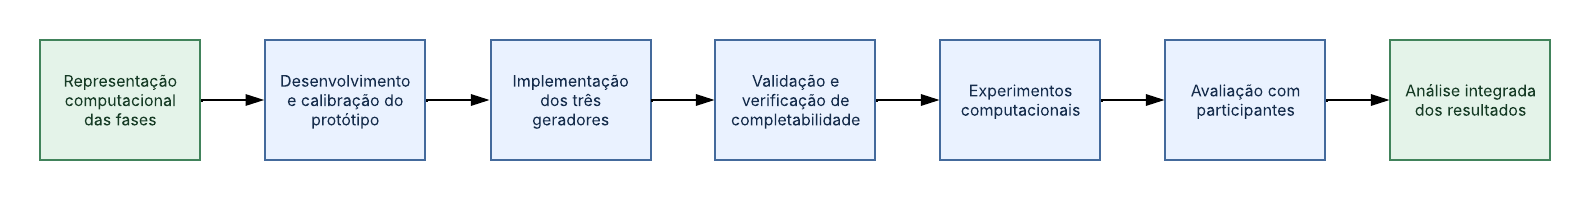
\includegraphics[width=0.9\textwidth]{imagens/FluxoMetodológicoFigura_1.png}
  \fonte{Autor (2026).}
\end{figure}

\begin{enumerate}
  \item \textbf{Representação computacional das fases:} 
  Cada fase conterá dez segmentos ordenados, cada qual com uma plataforma 
  estática e, no máximo, um obstáculo do tipo espinhos. Os atributos inteiros 
  serão largura $W_i\in[4,12]$, altura $H_i\in[0,6]$, vão $G_i\in[0,4]$, 
  presença de espinhos e posição $P_i$, em grade de 16 pixels. As alturas 
  serão medidas para cima a partir de uma referência, com $|H_{i+1}-H_i|\leq3$; 
  as posições horizontais obedecerão a $X_{i+1}=X_i+W_i+G_i$, com $X_1=0$ e $G_{10}=0$. 
  Os segmentos inicial e final não terão espinhos. Quando presentes nos 
  segmentos intermediários, ocuparão uma célula, com $1\leq P_i\leq W_i-2$; 
  quando ausentes, $P_i=0$. A primeira plataforma conterá a posição inicial 
  do personagem e a última, uma região de chegada.

  \item \textbf{Desenvolvimento e calibração do protótipo:} 
  Será implementado um jogo em C e raylib, com modos interativo e automatizado, 
  compartilhando a mesma rotina de física e colisões. O personagem Ninja Frog 
  utilizará sprite de $32\times32$ pixels e caixa de colisão independente. 
  O movimento horizontal terá velocidade constante e controle aéreo; 
  o salto terá impulso inicial e gravidade reduzida durante a subida, 
  enquanto o botão estiver pressionado, até um limite de sustentação. O salto 
  exigirá contato com o chão e novo acionamento do botão, sem 
  \emph{coyote time} ou \emph{jump buffer}. Os valores iniciais serão: 
  atualização de 60 Hz, velocidade horizontal de 160 px/s, impulso de 
  $-300$ px/s, gravidades normal e reduzida de 900 e 450 px/s$^2$, 
  sustentação de 0,20 s, caixa do personagem de $12\times24$ pixels e 
  velocidade máxima de queda de 600 px/s. Cenários de referência testarão 
  saltos, desníveis e colisões; eventuais ajustes serão documentados e 
  congelados antes dos experimentos definitivos.

  \item \textbf{Implementação dos geradores:} 
  o gerador \emph{aleatório} 
  sorteará uniformemente atributos dentro das restrições comuns, com 
  probabilidade de 40\% de espinhos em cada segmento intermediário. 
  O gerador \emph{baseado em regras} construirá a fase da esquerda para a 
  direita, com desnível máximo de duas unidades, vão máximo de duas unidades 
  em subidas, proibição de espinhos consecutivos e reserva de duas células 
  livres antes dos espinhos ($2\leq P_i\leq W_i-2$); a probabilidade inicial
  de espinhos será de 40\%, condicionada às regras. Nenhum dos dois consultará
  o simulador durante a construção. O \emph{algoritmo genético} utilizará 
  indivíduos com dez segmentos, população de 30, 50 ciclos de reprodução, 
  torneio de três, cruzamento em um ponto com probabilidade de 80\%, 
  mutação de um atributo com probabilidade de 10\% por segmento e 
  elitismo de dois indivíduos. Após os operadores, violações estruturais 
  serão reparadas sem consulta ao simulador. O limite será de 1.530 
  avaliações de aptidão por execução, incluindo a população inicial, 
  com reutilização de avaliações idênticas quando possível. A aptidão 
  será $F(L)=0{,}7C(L)+0{,}3P(L)$, sendo $C(L)=1$ apenas para conclusão 
  encontrada e reproduzida, e $P(L)$ o progresso horizontal máximo 
  normalizado entre início e chegada, limitado a $[0,1]$. Uma busca 
  inconclusiva não comprovará impossibilidade.

  \begin{figure}[htb]
  \centering
  \caption{Etapas do algoritmo genético empregado na geração das fases.}
  \label{fig:figura-2}
  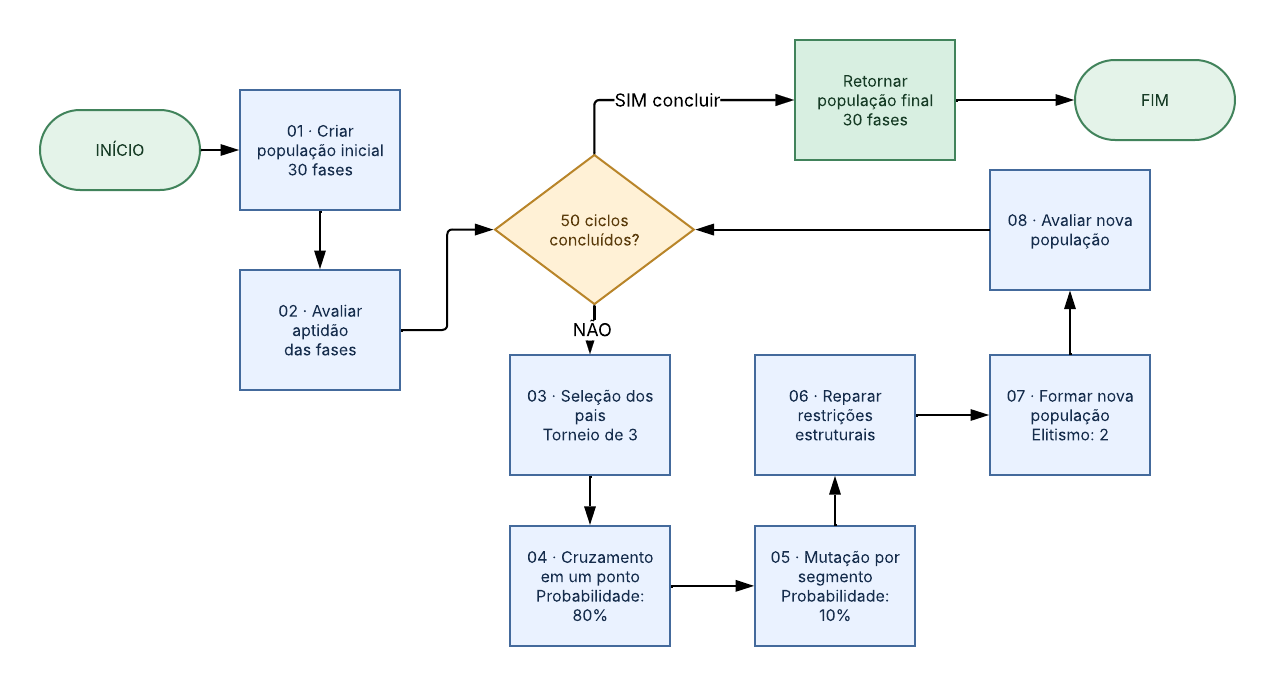
\includegraphics[width=0.75\textwidth]{imagens/FluxogramaAlgoritmoGenetico50ciclosFigura_2.png}
  \fonte{Autor (2026).}
  \end{figure}

  \item \textbf{Validação e completabilidade:} 
  inicialmente, serão verificados
  os limites dos atributos, os desníveis, as posições dos obstáculos e a 
  consistência dos segmentos. Depois, um simulador por busca em largura (BFS) 
  explorará estados com posição, velocidades, contato com o chão, estado e 
  duração do botão de salto e sobrevivência. As seis ações combinarão esquerda,
  parado ou direita com salto pressionado ou solto, mantidas por seis passos 
  físicos de $1/60$ s, com colisões verificadas a cada passo. A chave de 
  estados visitados discretizará posições em 4 pixels, velocidade vertical 
  em intervalos de 32 px/s, velocidade horizontal por direção e sustentação 
  em intervalos de 0,1 s, preservando as condições booleanas. O limite será 
  de 10.000 estados expandidos por fase. A busca registrará 
  \emph{sucesso reproduzido}, \emph{esgotamento sem sucesso no modelo explorado} 
  ou \emph{inconclusão por orçamento}. A morte ocorrerá por espinhos; 
  serão descartadas trajetórias cuja hitbox ultrapasse 128 pixels abaixo da 
  plataforma mais baixa ou 128 pixels além dos limites horizontais da fase. 
  A chegada será uma região de $16\times32$ pixels sobre a extremidade direita 
  da última plataforma. Sequências bem-sucedidas serão reproduzidas desde o 
  início para confirmação. O esgotamento da BFS não será interpretado como 
  prova de impossibilidade na física contínua.

  \begin{figure}[htb]
  \centering
  \caption{Procedimento de verificação automatizada de completabilidade por busca em largura.}
  \label{fig:figura-3}
  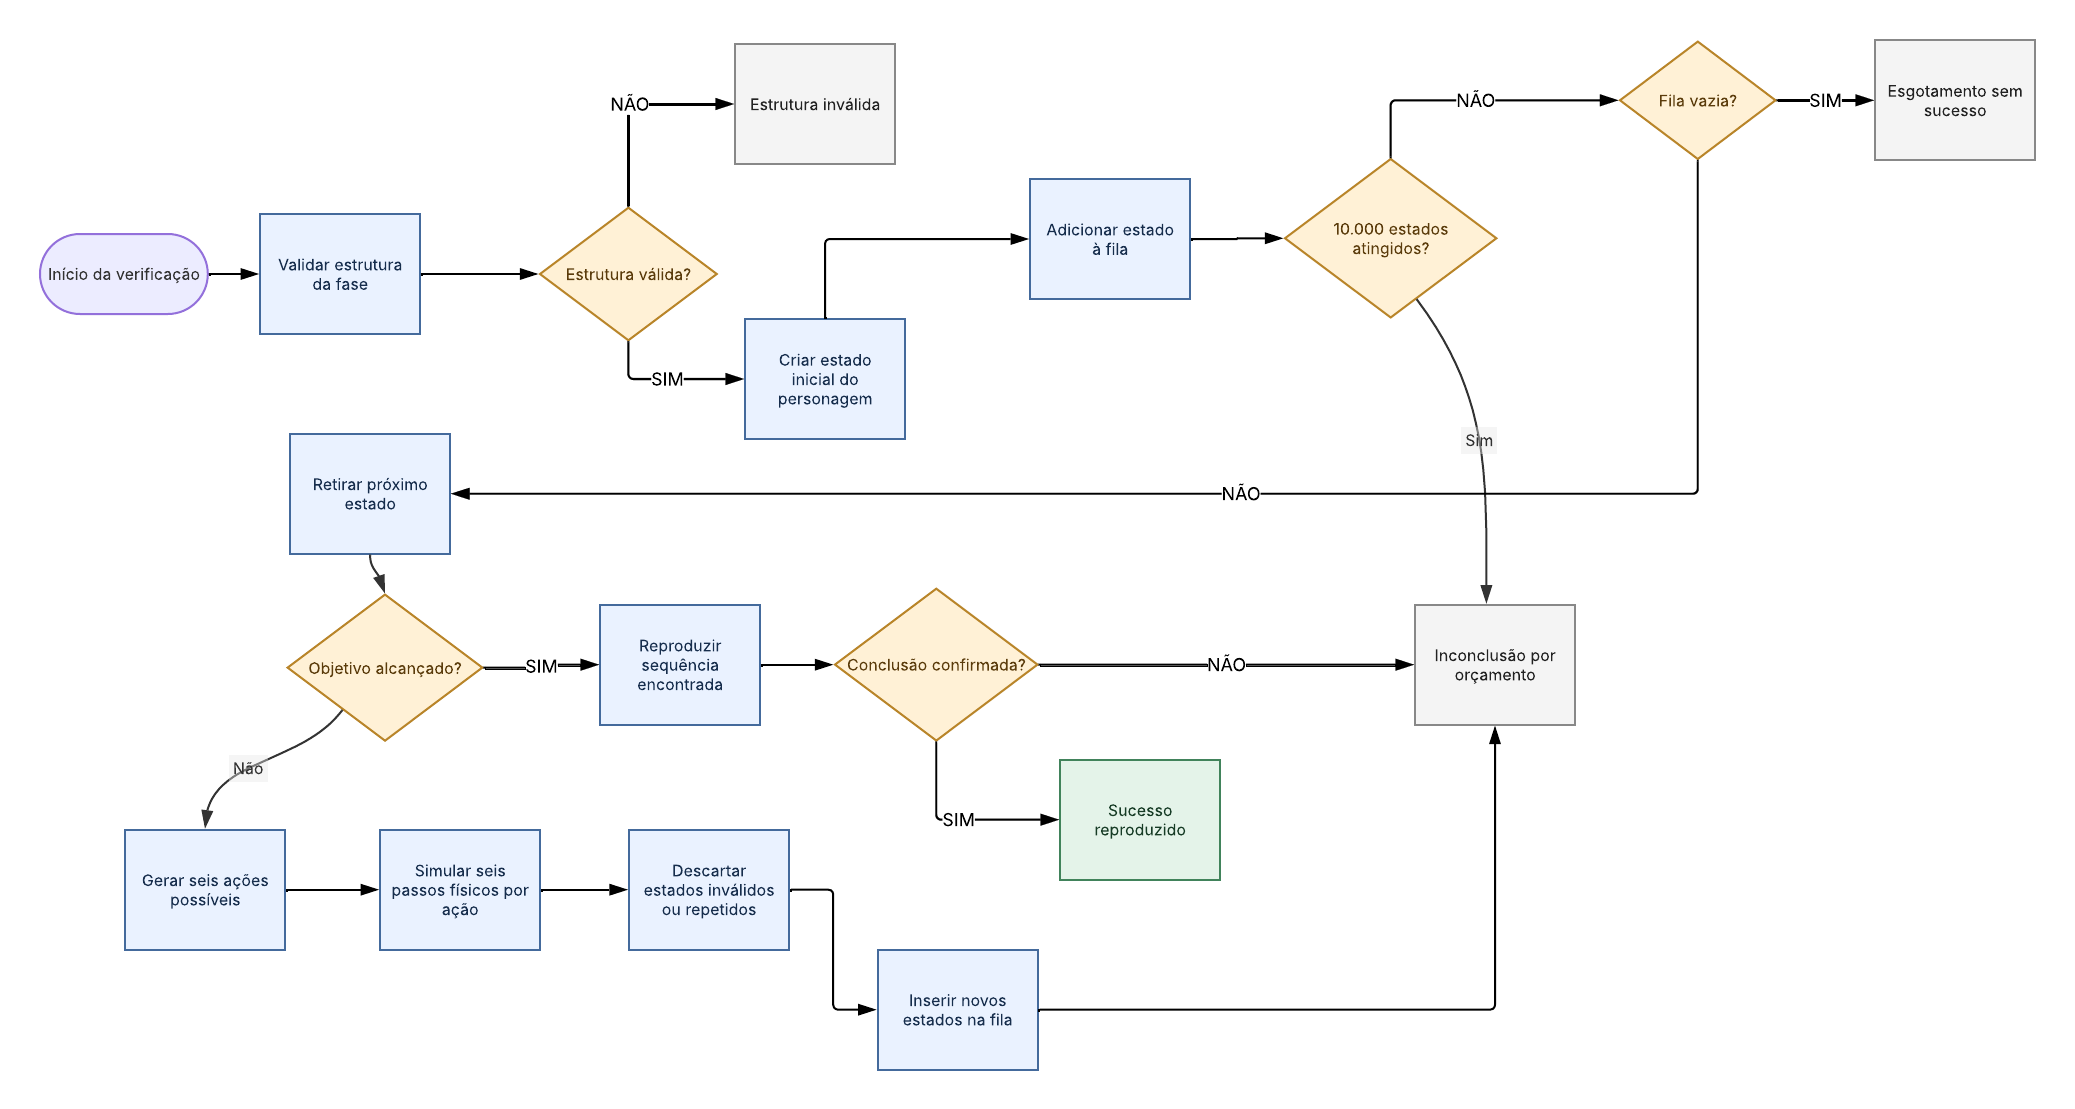
\includegraphics[width=0.95\textwidth]{imagens/FluxogramaVerificacaoFaseFigura_3.png}
  \fonte{Autor (2026).}
  \end{figure}

  \item \textbf{Experimentos computacionais:} 
  serão realizadas 30 execuções independentes por estratégia, com 
  sementes registradas e 30 fases finais por execução, totalizando 2.700 
  fases finais. No algoritmo genético, as 30 fases serão a população final, 
  inclusive possíveis duplicatas. Serão registrados candidatos produzidos, 
  avaliações e estados expandidos, validade estrutural, sucesso demonstrado, 
  inconclusão, tempo de construção, otimização, avaliação e tempo total, sem 
  contagem dupla. As taxas terão como denominador as 30 fases finais por 
  execução. A diversidade será a média das distâncias entre os 435 pares de 
  fases finais, com
  \begin{equation}
  D(A,B)=\frac{D_W+D_H+D_G+D_O}{4},\qquad
  \operatorname{Div}(S)=\frac{2}{n(n-1)}\sum_{i<j}D(L_i,L_j),\quad n=30.
  \end{equation}
  As diferenças de largura, altura e vão serão médias das diferenças 
  absolutas por segmento, normalizadas respectivamente por 8, 6 e 4; para o 
  vão serão considerados os nove primeiros segmentos. Para espinhos, a 
  diferença por segmento intermediário será zero se ambos estiverem ausentes, 
  um se apenas um estiver presente ou a diferença absoluta entre posições 
  relativas $r_i=(P_i-1)/(W_i-3)$ quando ambos estiverem presentes; $D_O$ 
  será a média dos oito segmentos intermediários. Também serão registradas 
  fases únicas e densidade de espinhos. Três execuções piloto por estratégia 
  verificarão custos, registros e inconclusões; seus dados não integrarão a 
  coleta definitiva. Os parâmetros serão congelados após o piloto.

  \begin{figure}[htb]
  \centering
  \caption{Organização dos experimentos computacionais e das métricas de comparação.}
  \label{fig:figura-5}
  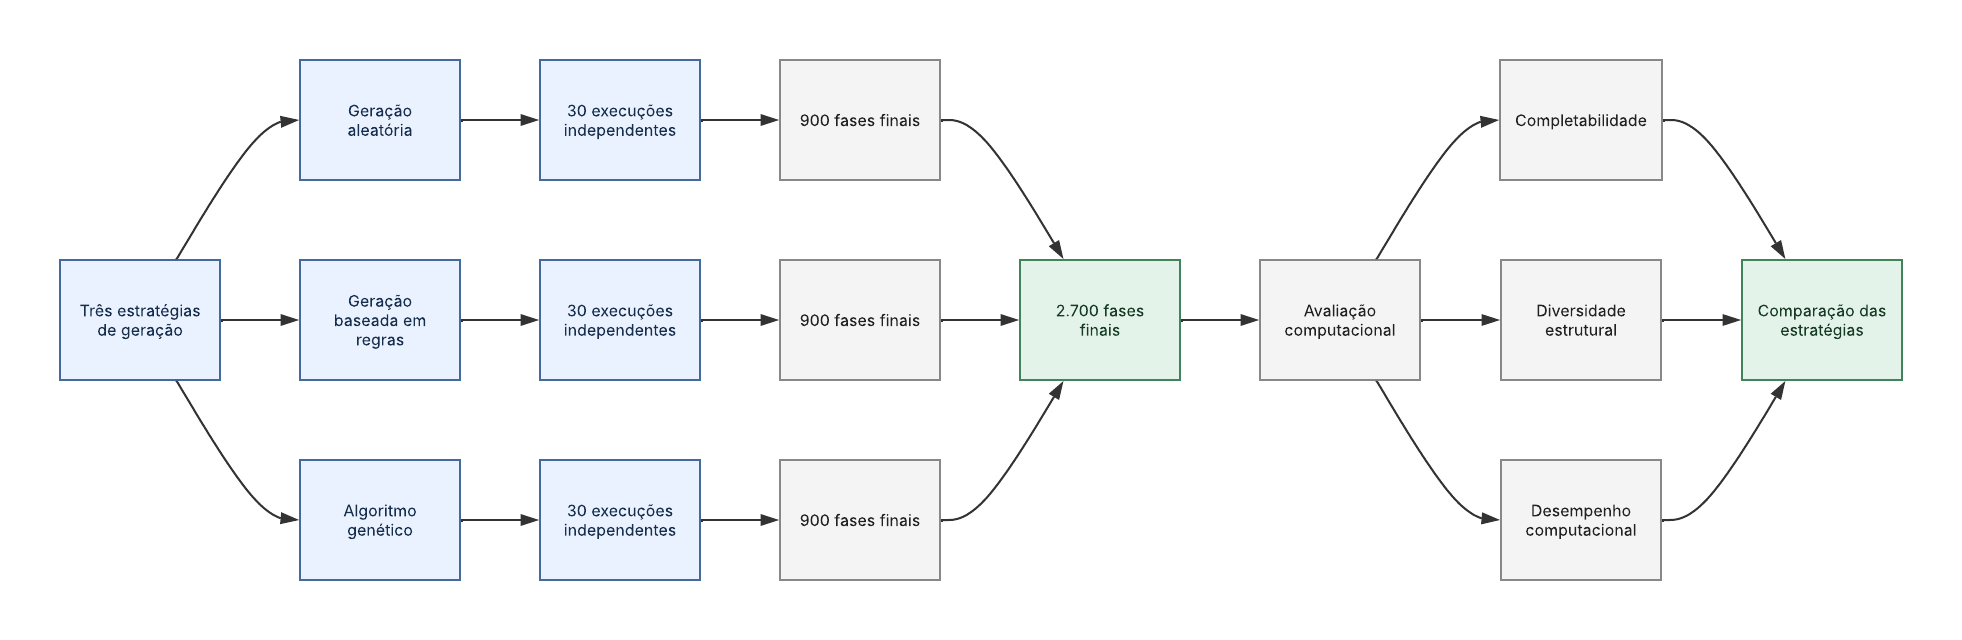
\includegraphics[width=0.95\textwidth]{imagens/Fluxograma Avaliacao Computacional EstrategiasGeracaoFigura_5.png}
  \fonte{Autor (2026).}
  \end{figure}
  
  \item \textbf{Avaliação com participantes:} 
  a meta será de 24 adultos voluntários, recrutados por conveniência. 
  Após uma fase comum de treinamento, cada participante jogará seis fases: 
  duas por estratégia, com limite de três minutos por fase e tentativas 
  múltiplas. Serão sorteadas, com semente registrada, duas fases distintas e 
  com conclusão demonstrada por estratégia; todos jogarão as mesmas seis fases. 
  A seleção ocorrerá antes das sessões, sem escolha manual por aparência. 
  As seis ordens de apresentação das estratégias serão distribuídas igualmente 
  (quatro participantes por ordem), alternando-se também a ordem interna das 
  duas fases. Serão registrados conclusão, tempo, tentativas e mortes. Após 
  cada bloco de duas fases, serão aplicados cinco itens Likert de 1 a 5 sobre 
  dificuldade, diversão, satisfação, clareza e variedade; ao final, 
  uma pergunta aberta solicitará pontos positivos e negativos. A avaliação 
  humana será exploratória, pois apenas duas fases fixas representarão 
  cada estratégia.

  \begin{figure}[htb]
  \centering
  \caption{Etapas da sessão de avaliação da experiência dos participantes.}
  \label{fig:figura-4}
  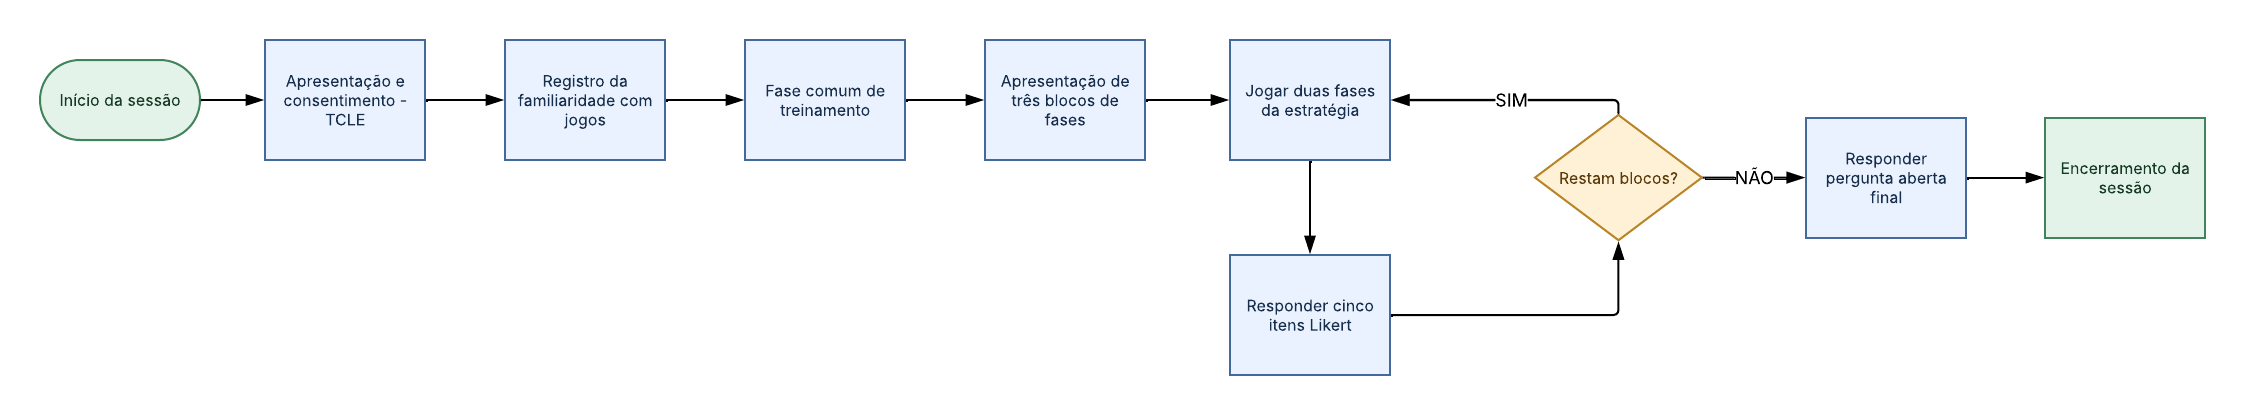
\includegraphics[width=0.95\textwidth]{imagens/FluxogramaProcedimentoExperimentalFigura_4.png}
  \fonte{Autor (2026).}
  \end{figure}

  \item \textbf{Análise dos resultados:} 
  a unidade principal de análise computacional será a execução independente, 
  agregando suas 30 fases para evitar pseudorreplicação. Serão apresentadas 
  média, desvio-padrão, mediana, dispersão e intervalos de confiança de 95\%.
  As comparações considerarão os pressupostos dos dados: ANOVA, ANOVA de Welch
  ou alternativas não paramétricas/de reamostragem, com correção para múltiplas 
  comparações, tamanhos de efeito e nível de significância de 5\%. Para os 
  itens Likert, serão respeitadas as medidas repetidas, considerando o teste 
  de Friedman e comparações pareadas com ajuste de Holm. Tempos interrompidos 
  pelo limite não serão tratados como tempos de conclusão. As respostas abertas 
  serão organizadas em categorias temáticas. A interpretação considerará 
  conjuntamente completabilidade, diversidade, custo e experiência, sem 
  presumir superioridade global de uma estratégia.

\end{enumerate}

% 3.3 Ambiente e Participantes
\section{Ambiente e Participantes}
\label{sec:ambiente-participantes}

Todas as estratégias utilizarão o mesmo executável, modelo físico e critérios 
de avaliação, em modo sem renderização. A avaliação humana terá como meta 24 
participantes adultos com diferentes níveis de familiaridade com jogos de 
plataforma 2D, registrada antes das sessões. O recrutamento será por 
conveniência e as sessões utilizarão controles e instruções padronizados. 
O número previsto é uma meta operacional, não garantia de poder estatístico.

% 3.5 Tecnologias e ferramentas (para projetos de software)
\section{Tecnologias e Ferramentas}
\label{sec:tecnologias-ferramentas}

O Quadro~\ref{qua:tecnologias} apresenta as ferramentas previstas. 
A linguagem C e a raylib permitirão compartilhar a física entre o jogo e o simulador; 
CMake e Git apoiarão a reprodutibilidade do desenvolvimento; 
arquivos CSV registrarão os dados dos experimentos.

\begin{table}[htb]
\caption{Tecnologias e ferramentas previstas}
\label{qua:tecnologias}
\begin{tabularx}{\textwidth}{lXl}
  \toprule
  \textbf{Tecnologia/Ferramenta} & \textbf{Função no Projeto} & \textbf{Categoria} \\
  \midrule
  C & Protótipo, geradores, física e simulador & Programação \\
  raylib & Renderização e comandos do jogador & Biblioteca gráfica \\
  CMake & Configuração da compilação & Construção \\
  Git & Versionamento de código e parâmetros & Versionamento \\
  CSV & Registro de sementes, métricas e resultados & Dados \\
  \bottomrule
\end{tabularx}
\fonte{Elaborado pelo autor (\oano).}
\end{table}

% 3.5 Considerações éticas
\section{Considerações Éticas}
\label{sec:consideracoes-eticas}

Esta pesquisa envolve seres humanos e, portanto, será submetida
ao Comitê de Ética em Pesquisa (CEP) da instituição, conforme
a Resolução CNS 466/2012. Os participantes serão informados
sobre os objetivos da pesquisa e assinarão o Termo de
Consentimento Livre e Esclarecido (TCLE) antes da coleta
de dados. A identidade dos participantes será mantida em
sigilo em todas as etapas da pesquisa.
